%%%%%%%%%%%%%%%%%%%%%%%%%%%%%%%%%%%%%%%%%%%%%%%%%%%%%%%%%%%%%%%%%%%%%%%%%%%%%
%%
%% Classes disponibles :
%%	- times : utilisation de la police Times par défaut.
%%	- these, sujthese, projthese, memoire, essai, rapport : pour
%%		générer la page de garde en fonction du type document.
%%	- french, english : selon la langue dans laquelle doit
%%		être rédigé le document.
%%  - ieee, apa : style des références bibliographiques
%%  - twoside : alternance des marges pour impression recto/verso
%%    vous devez décommenter la ligne 22 si vous utilisez cette classe
%%
%%%%%%%%%%%%%%%%%%%%%%%%%%%%%%%%%%%%%%%%%%%%%%%%%%%%%%%%%%%%%%%%%%%%%%%%%%%%%%

\documentclass[12pt,times,these,french,apa]{uqac}

%%%%%%%%%%%%%%%%%%%%%%%%%%%%%%%%%%%%%%%%%%%%%%%%%%%%%%%
%%
%% Décommenter la ligne suivante avec l'utilisation de
%% la classe "twoside"
%%
%%%%%%%%%%%%%%%%%%%%%%%%%%%%%%%%%%%%%%%%%%%%%%%%%%%%%%%
% \raggedbottom

%%%%%%%%%%%%%%%%%%%%%%%%%%%%%%%%%%%%%
%%
%% Préciser l'emplacement du fichier
%% contenant les acronymes.
%%
%%%%%%%%%%%%%%%%%%%%%%%%%%%%%%%%%%%%%
\acrolistpath{assets/acro}

%%%%%%%%%%%%%%%%%%%%%%%%%%%%%%%%%%%%%%%%%%%%%%%%%%%%%%%%
%%
%% Toutes les images utilisées doivent se trouver dans
%% le répertoire "assets/figure".
%%
%%%%%%%%%%%%%%%%%%%%%%%%%%%%%%%%%%%%%%%%%%%%%%%%%%%%%%%%
\graphicspath{{assets/figures/}}

%%%%%%%%%%%%%%%%%%%%%%%%%%%%%%%%%%%%
%%
%% Packages utilisateurs ci-dessous:
%%
%%%%%%%%%%%%%%%%%%%%%%%%%%%%%%%%%%%%
\usepackage{graphicx}
\usepackage{soul, color, xcolor, soulutf8}

\usepackage{xargs}                      % Use more than one optional parameter in a new commands

\usepackage{tikz}
\usetikzlibrary{babel}
\usepackage{chemfig}
\usepackage{chemnum}
\usepackage{acronym}  
\usepackage[europeanresistors,americaninductors]{circuitikz}
\usepackage{tikz-feynman}
\usepackage{hyperref}
\usepackage{algorithmic}

\usepackage[colorinlistoftodos,prependcaption,textsize=tiny]{todonotes}

\graphicspath{{assets/figures/}}


\hypersetup{
  colorlinks=true,
  linkcolor=black,
  urlcolor=[rgb]{0,0.501,0.674},
  breaklinks=true,
  citecolor=[rgb]{0,0.501,0.674},
  bookmarks=true
}
\SetKwInput{KwEntree}{Entrées}
\SetKwInput{KwSortie}{Sortie}
% Algorithm packages
%\usepackage{algorithm}  % or \usepackage{algorithm2e} depending on what you need
%\usepackage{algorithmic}  % if you want to write pseudo-code
%%%%%%%%%%%%%%%%%%%%%
%%
%% Césures manuelles
%%
%%%%%%%%%%%%%%%%%%%%%
% \hyphenation{con-nection con-nue con-cep-tion}

%%%%%%%%%%%%%%%%%%%%%%%%%%%%%%%%
%%
%% Gestion des lignes orphelines
%%
%%%%%%%%%%%%%%%%%%%%%%%%%%%%%%%%
\widowpenalty10000
\clubpenalty10000
\begin{document}


%%%%%%%%%%%%%%%%%%%%%%%%%%%%%
%%
%% Titre, auteur et programme
%%
%%%%%%%%%%%%%%%%%%%%%%%%%%%%%

\title{Un titre qui représente la contibution principale du mémoire}
\author{Nom de l'étudiant.e}
\programme{ingénierie}

%%%%%%%%%%%%%%%%%%%%%%%%%%%%%%%%%%%%%
%%
%% S’il y a lieu, indiquer le profil
%% ou la concentration du programme
%%
%%%%%%%%%%%%%%%%%%%%%%%%%%%%%%%%%%%%%
%\concentration{profil recherche}

%%%%%%%%%%%%%%%%%%%%%%%%%%%%%%%%%%%%%%%%%%%%
%%
%% Par défaut l'année courante est utilisée.
%% Pour spécifier une autre année :
%%
%%%%%%%%%%%%%%%%%%%%%%%%%%%%%%%%%%%%%%%%%%%%
%\degreeyear{2018}
% Ajout d'une page vide avec les mêmes dimensions que les autres pages
\newpage
\null
\thispagestyle{empty} % Pas de numéro de page sur la page vide
\newpage

% Modifier les marges spécifiquement pour la page de garde
\newgeometry{a4paper,left=35mm, right=25mm, top=25mm, bottom=25mm} % Par exemple, des marges réduites

\maketitle


%%%%%%%%%%%%%%%%%%%%%
%%
%% Page préliminaires
%%
%%%%%%%%%%%%%%%%%%%%%
\begingroup
\singlespacing
\opening
%\pagestyle{empty}

\begin{abstract}
Ici, c'est normalement en \hl{anglais}

Afin de parvenir à une ... Dans ce contexte, les systèmes ... \par

Écrire environ 300 mots:
\begin{itemize}
\item contexte et problématique (3 phrases)
\item objectifs (2 phrases) 
\item hypothèses (2 phrases)
\item méthode principale (2 phrases) 
\item résultat significatif principal (2 phrases) 
\item conclusion et travaux futures (2 phrases) 
\end{itemize}


\textbf{Mots clés :} \textbf{Optimisation, Collaboration humain-robot, Approche globale, Algorithmes génétiques...}

\end{abstract}

\begin{resume}

Ici, c'est normalement en français

Afin de parvenir à une ... Dans ce contexte, les systèmes ... \\

Écrire environ 300 mots:\\
- contexte et problématique (3 phrases)\\
- objectifs (2 phrases)\\
- hypothèses (2 phrases)\\
- méthode principale (2 phrases)\\
- résultat significatif principal (2 phrases)\\
- conclusion et travaux futures (2 phrases)\\


\textbf{Mots clés :} \textbf{Optimisation, Collaboration humain-robot, Approche globale, Algorithmes génétiques...}


\end{resume}


%%%%%%%%%%%%%%%%%%%%%%%%%%%%%%%%%%%%%%%%%%%%%%%%%%%%%%%%%%
%%
%% Si vous écrivez un document en anglais,
%% il sera nécessaire de fournir un résumé en Français :
%%
%%%%%%%%%%%%%%%%%%%%%%%%%%%%%%%%%%%%%%%%%%%%%%%%%%%%%%%%%%
% Ajouter un espace avant l'entrée "Table des Matières" dans la table des matières
\addtocontents{toc}{\vspace{0.3cm}} % Ajustez la valeur pour plus ou moins d'espace

% Ajoutez une entrée pour "Table des Matières" dans la table des matières elle-même
\addcontentsline{toc}{chapter}{\bfseries\MakeUppercase{Table des Matières}}

\tableofcontents
\cleardoublepage
\listoftables
\listoffigures
\listofacro

\begin{dedic}
\begin{center}
\it \Large
   \vspace{5mm}
Je dédie ce mémoire \\
\vspace{5mm}
{\bf À mes chers parents} \\
\vspace{5mm}
À ceux qui se sentiront honorés ..., \\
\vspace{0.5mm}
en l’honneur .... \\
\vspace{0.5mm}
tout au long ... \\
\vspace{4mm}
Aucun mot, aucune dédicace ... \\
\vspace{0.5mm}
mon admiration et ma ... \\
\vspace{0.5mm}
sacrifices qu’ils ... \\
\end{center}
\vspace{4mm}
\vspace{8mm}
\begin{flushright}
     {\bf Nom de l'étudiant.e}
\end{flushright}
\newpage
\thispagestyle{empty}
\end{dedic}



\begin{ack}
%\setstretch{1.5}
Je souhaite dédier cette page...\par
Support financier de ... \par
Ce travail a été réalisé au sein du Laboratoire d'Automatique et de Robotique Interactive (LAR.i) de l’Université du Québec à Chicoutimi (UQAC), sous la direction de Monsieur Martin Otis, professeur au département des sciences appliquées....\par
Je tiens à exprimer ma profonde gratitude...\par
En conclusion, ...\par

\end{ack}

\endgroup
\include{content/avant_propos}

%%%%%%%%%%%%%%%%%%%%%
%%
%% Document principal
%%
%%%%%%%%%%%%%%%%%%%%%
% \pagestyle{fancy}
\doublespacing
\maincontent
\begin{introduction}
Au cours des dernières années, ...
\end{introduction}

\chapter{MISE EN CONTEXTE}
\label{chap:chap_1}
%\section{introduction}
\listoftodos[Notes]%ceci permet d'afficher la liste dee commentaires du professeur

\section*{Introduction}

Les progrès récents ...

\section{Contexte de la recherche}
Le contexte de la recherche doit être présenté de manière à fournir une compréhension approfondie du sujet étudié. Il doit inclure une revue de la littérature pertinente, en mettant en évidence les travaux antérieurs et les lacunes dans la recherche existante. Le contexte doit également expliquer l'importance du sujet de recherche et justifier la nécessité de mener cette étude. Il est important de présenter le contexte de manière claire et concise, en évitant les détails inutiles et en se concentrant sur les aspects les plus pertinents pour la recherche. Le contexte doit être présenté de manière logique, en utilisant des transitions pour relier les différentes idées et en fournissant des exemples concrets pour illustrer les points clés. Il est également important de s'assurer que le contexte est aligné avec les objectifs de recherche et la problématique posée dans l'introduction, en fournissant une base solide pour la suite du document.
La revue de la littérature présenté dans cette section est courte et directement centré sur le projet de recherche de manière à présenter les travaux les plus pertinents pour le projet de recherche et permette l'identification des lacunes dans la recherche existante et être en mesure d'écrire adéquatement une problématique claire.

\section{Problématique}

La rédaction d'une problématique doit être claire, concise et bien structurée. La problématique annoce le vérou scientifique du projet de recherche, en identifiant les lacunes dans la littérature existante de la section précédente et en présentant les questions de recherche qui seront abordées dans le document. Il est important de formuler la problématique de manière à ce qu'elle soit compréhensible pour les lecteurs, en évitant le jargon technique ou les termes ambigus. La problématique doit être présentée de manière logique, en utilisant l'introduction générale du sujet et de l'analyse des travaux antérieurs et des lacunes précédemment identifiées. La problématique adresse les questions de recherche spécifiques qui seront abordées dans le document. Il est également important de s'assurer que la problématique est alignée avec les objectifs de recherche et qu'elle contribue de manière significative à la compréhension du sujet étudié.

L'introduction  des...
La problématique centrale de ce projet de recherche réside...


\section{Objectifs}
Les objectifs doivent être clairement définis et alignés avec la problématique de recherche. Ils doivent être spécifiques, mesurables, atteignables, pertinents et temporellement définis (SMART). Les objectifs doivent être formulés de manière à guider la recherche et à fournir une base pour l'évaluation des résultats. Ils doivent également être présentés de manière logique, en commençant par les objectifs généraux et en les décomposant en objectifs spécifiques. Il est important de s'assurer que les objectifs sont réalisables dans le cadre du projet de recherche et qu'ils contribuent de manière significative à la compréhension du sujet étudié. 

L'objectif principal de ce projet de recherche est de déterminer...

\subsection{Conseils de rédaction}

Pour enlever le contour de l'image, on peut utiliser les paramètres trim et clip. La commande est :\par

\begin{verbatim}
includegraphics[trim={A cm B cm D cm E cm},clip, width=\linewidth],
\end{verbatim}
avec: \par
trim=A:left B:bottom C:right D:top\par 

Voici un exemple de figure côte à côte:

\begin{figure}[!htbp]
\centering
    \begin{minipage}{0.45\linewidth}
        \centering
        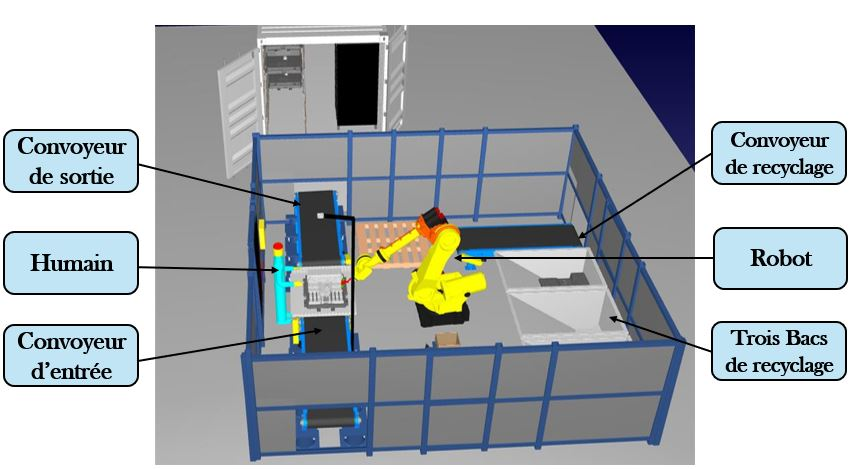
\includegraphics[width=\textwidth]{usine.JPG}
        \caption{Example of the hybrid mobile robot with UR5 serial manipulator for the use case study. Source of 3D files, CC-BY \cite{vanel}}\label{fig:robotUR5}
    \end{minipage}
    \begin{minipage}{0.45\linewidth}
        \centering
        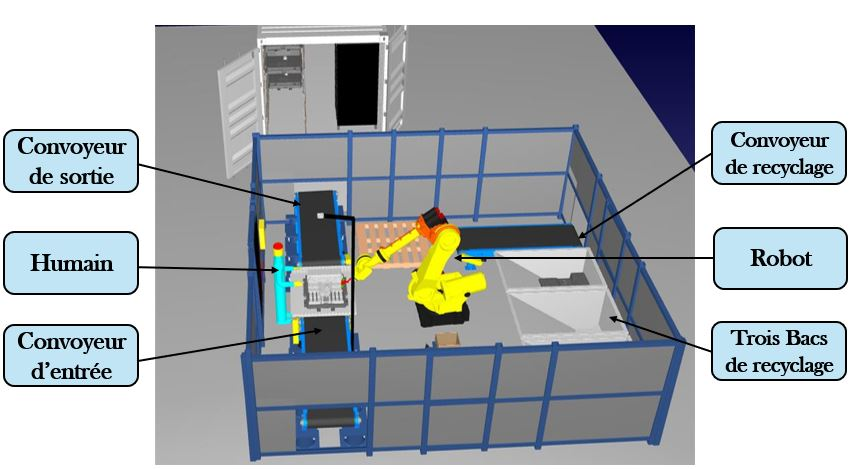
\includegraphics[width=\textwidth]{usine.JPG}
        \caption{3D simulation of an electrical substation on Gazebo in ROS. Source of 3D files, CC-BY \cite{vanel}.}\label{fig:3DSousStation}
    \end{minipage}
\end{figure}

\subsubsection{Utilisation des accronymes}
Pour les définitions des acronymes, on doit les ajouter manuellement, par exemple pour \ac{BMS}.
Le même principe s'applique pour \ac{TSP}.
À chaque fois que l'acronyme est utilisé, on doit prendre la commande \ac{TSP}, après l'avoir défini à la première référence.

\subsubsection{Notes de bas de page}

Vous pouvez utiliser les notes de bas de page pour inclure un lien\footnote{\url{https://www.uqac.ca}} en rapport avec votre texte, ou pour donner plus de précisions\footnote{Cette note de bas de page propose plus d'informations}.

\subsubsection{Exemple de listes}
\label{subsec:subsec_list}

\begin{enumerate}
  \item {\bf premier point (gras) ;}
  \item {\em second point (italique) ;}
  \item {\Large troisième point (gros) ;}
      \begin{enumerate}
          \item {\small premier sous-point en petit}
          \item {\tiny second sous-point (petit)}
          \item {\Huge troisième sous-point (très gros)}
      \end{enumerate}
  \item[$\bullet$] {\sf point avec une puce (sans serif)}
  \item[$\circ$] {\sc point avec un autre style de puce (petites lettres capitales)}
\end{enumerate}


\section*{Conclusion}
\label{sec:sec_examples_chap_1}

La conclusion n'est pas une discussion. Elle doit être structurée de manière à résumer les points clés abordés dans le chapitre, à présenter les implications de ces points pour la suite du document et à faire le lien avec les chapitres suivants.

La conclusion doit comprendre une synthèse des points clés abordés dans le chapitre, ainsi que les implications de ces points pour la suite du document. Elle doit également faire le lien avec les chapitres suivants en présentant les questions de recherche qui seront abordées dans les sections suivantes.

La conclusion doit être concise et claire, en évitant de répéter les informations déjà présentées dans le chapitre. Elle doit plutôt se concentrer sur les implications et les perspectives futures de la recherche présentée dans le chapitre.

Il est requis de réaliser un rappel des hypothèses afin de la confirmer ou des les infirmer, ainsi que de présenter les travaux futurs qui seront réalisés dans les sections suivantes.

Ce projet de recherche vise à résoudre...

\newpage

\chapter{revue de littérature}
\label{chap:chap_2}
\section*{Introduction}
La technologie...
Sujet amené
Sujet posé\todo{commentaire du professeur}
Sujet divisé

\section{revue de littérature}
Le processus de reconditionnement, soutenu par la technologie de collaboration humain-robot, joue un rôle de plus en plus important, contribuant au développement économique tout en réduisant considérablement la pression sur l'environnement \cite{wu2024}.

La table \ref{relatedworks} présente des travaux similaires comparés à l'approche suggérée...

\begin{table}[!htbp]
\centering
\caption{Un titre de tableau}
\label{relatedworks}
\large % Augmentation subtile de la taille de la police
\renewcommand{\arraystretch}{1.7} % Augmente l'espacement vertical
\resizebox{\linewidth}{!}{
\begin{tabular}{|>{\centering\arraybackslash}m{2.2cm}|>{\centering\arraybackslash}m{1.9cm}|>{\centering\arraybackslash}m{2.2cm}|>{\centering\arraybackslash}m{2.6cm}|>{\centering\arraybackslash}m{2.6cm}|>{\centering\arraybackslash}m{2.1cm}|>{\centering\arraybackslash}m{2.2cm}|>{\centering\arraybackslash}m{2.0cm}|>{\centering\arraybackslash}m{2.6cm}|}
\hline
\textbf{Approche} & \textbf{Tâches fixes} & \textbf{Humain entité non-prévisible} & \textbf{Distribution non fixe du temps} & \multicolumn{2}{>{\centering\arraybackslash}m{4.4cm}|}{\textbf{Contraintes}} & \multicolumn{2}{>{\centering\arraybackslash}m{4.4cm}|}{\textbf{Approche}} & \textbf{Formulation globale du problème} \\
\cline{5-6} \cline{7-8}
 &  &  &  & \textbf{Coopération} & \textbf{Exclusion} & \textbf{Prédictive} & \textbf{Réactive} &  \\
\hline
Wu et al. 2023 \cite{TengfeiWu2023} &  &  &  & X &  & X &  & X \\
\hline
Ke et al. 2020 \cite{Qingdike2020} & X  &  &  & X &  & X &  & X \\
\hline

Vanel et al.2024 \cite{vanel} & X & X & X & X & X & X & X & \\
\hline
\textbf{Notre approche} & X & X & X & X & X & X & X & X\\
\hline
\end{tabular}
}
\end{table}
Dans les configurations...


\section{Hypothèses}
Ce projet de recherche repose sur X hypothèses...

\section{Conclusion}

Retour sur les objectifs de ce chapitre
Faisabilité et perspective
Présentation du prochain chapitre


\chapter{Méthodologie}
\label{chap:chap_3}
\section*{Introduction}
Sujet amené
Sujet posé
Sujet divisé


\section{Description et formulation du problème}
Présenter les sous-sections...
\subsection {Architecture proposée}
Dans ce projet, ... La figure \ref{usine} donne un aperçu de l’installation dans l’environnement RoboDK, montrant la batterie dans l’espace de travail.


\begin{figure}[!htbp]
    \centering
    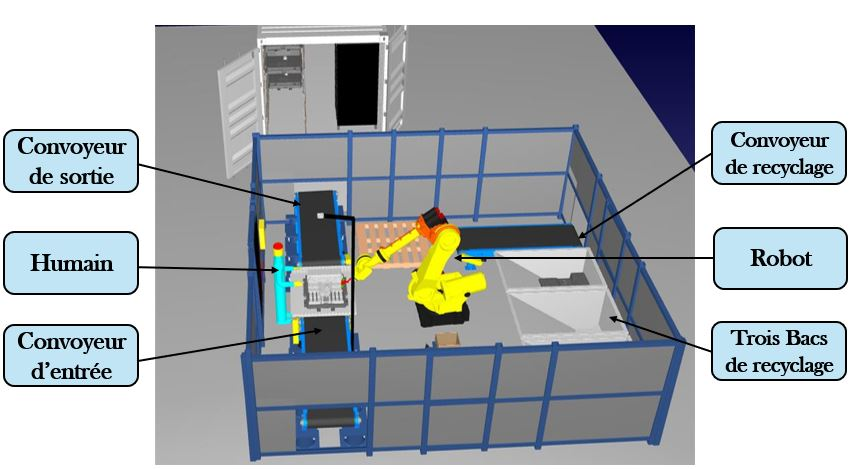
\includegraphics[width=\linewidth]{usine.JPG}
    \caption{Usine de démontage d’une batterie NISSAN Leaf \cite{vanel}}
    \label{usine}
\end{figure} 




\subsection{Une autre sous-section}

\section{Une section}
Présenter les sous-sections... 



\subsection{Objectifs et contraintes}

L'équation (\ref{eq:time_matrix}) décrit...

\begin{equation}
T = \begin{pmatrix}
t_{11} & t_{12} & \cdots & t_{1n} \\
t_{21} & t_{22} & \cdots & t_{2n} \\
\vdots & \vdots & \ddots & \vdots \\
t_{n1} & t_{n2} & \cdots & t_{nn}
\end{pmatrix}
\label{eq:time_matrix}
\end{equation}

L'algorithme \ref{alg:generate_population1} présente...

\begin{minipage}{0.98\linewidth} % Réduire la largeur du cadre à 80% de la largeur de la page
\begin{algorithm}[H]
\caption{Algorithme de génération de la population initiale}
\label{alg:generate_population1}
    \KwEntree{Nombre de population, Nombre de tâches, Matrice de précédence }
  \KwSortie{Population initiale}
  Initialiser une liste vide pour stocker les chemins constituant la population \;
   \While{la taille de la population < au Nombre de population}{
    Générer un chemin aléatoire en respectant les contraintes de précédence \;
    \eIf{le chemin généré est unique et respecte les contraintes}{
     Ajouter le chemin à la population \;
     Continuer \;
     }{
     Ignorer le chemin \;
    }
   }
\end{algorithm}
\end{minipage}
\newline 
Pour améliorer la performance de l'algorithme...



\subsection{Mise en œuvre de l'algorithme génétique} 

\section{Conclusion}
Rappel des objectifs du chapitre
Indiquer l'atteinte des objectifs
Présenter le prochain chapitre


\chapter{Résultats et discussions}
\label{chap:chap_4}
\section*{Introduction}
Sujet amené
Sujet posé
Sujet divisé

\subsection{Résultat 1}
Pour évaluer 

\subsection{Résultat 2}
Pour évaluer 

\section{Discussion}


\section{Conclusion}
Rappel des objectifs du chapitre
Indiquer l'atteinte des objectifs
Présenter le prochain chapitre

\chapter{Résultats et discussions 2}
\label{chap:chap_5}
\section{Introduction}
Sujet amené
Sujet posé
Sujet divisé

\section{Résultat 2}


\section{Discussion}

\section{Conclusion}
Suite aux résultats obtenus dans ce chapitre, ...
Rappel des objectifs du chapitre
Indiquer l'atteinte des objectifs
Présenter le prochain chapitre
\begin{conclusion}

Les progrès récents...



\end{conclusion}


%%%%%%%%$%%%%
%%
%% Références
%%
%%%%%%%%%%%%%

%%%%%%%%%%%%%%%%%%%%%%%%%%%%%%%%%%%%%%%%%%%%%%%%%%%%%%%%%%
%%
%% Le fichier BibTeX contenant les références
%% doit se trouver dans le répertoire "assets/references".
%%
%%%%%%%%%%%%%%%%%%%%%%%%%%%%%%%%%%%%%%%%%%%%%%%%%%%%%%%%%%
\begingroup
\singlespacing

\bibliography{assets/references}

\endgroup
%%%%%%%%%%%
%%
%% Annexes
%%
%%%%%%%%%%%
%\appendix

\include{content/annexe_a}

\end{document}
